\section{Feststellung geeigneter Parameter}
\label{parameters}

Diese Arbeit soll sich im großen Maße mit der Ermittlung geeigneter Parameter für die Einschätzung der Fahrtauglichkeit beschäftigen. Dazu werden im Folgenden verschiedene Parameter aus im Abschnitt \ref{relatedWork} genannten Richtlinien genannt und erläutert. Im nächsten Schritt werden dann Möglichkeiten der Messung dieser Parameter aufgeführt. Daraus wird dann eine Auswahl von gut messbaren Parametern getroffen, auf welche sich dann in den folgenden Teilen dieser Arbeit stärker bezogen wird.
\subsection{Ermittlung der Parameter}

Die Richtlinie der Driver \& Vehicle Licensing Agency \cite{drivervehiclelicencingagency} führt bereits ein detaillierten Überblick von zu bewertenden Parametern auf:

\begin{multicols}{2}
\begin{itemize}
	\item Sehvermögen
	\item Visuelle Raumvorstellung
	\item Hörvermögen
	\item Aufmerksamkeit und Konzentration
	\item Gedächtnis
	\item Einsicht und Verständnis
	\item Urteilsfähigkeit
	\item Reaktionsfähigkeit
	\item Persönliche Organisation
	\item Fähigkeit zur Selbstüberwachung
	\item Sensitivität
	\item Körperliche Voraussetzungen
	\item Koordination
	\item Adaptive Strategien (Anpassungsfähigkeit)
\end{itemize}
\end{multicols}

Bei den Körperlichen Voraussetzung wird hierbei speziell auf die Muskelkraft und - kontrolle verwiesen. Die Begutachtungsleitlinien zur Kraftfahreignung \cite{begutachtungsrichtlinien} und die daraus abgeleiteten unterstützenden Testverfahren \cite{testverfahrenpsychometrischefahreignung} folgen im wesentlichen diesen Parametern, zählen aber die Belastbarkeit noch als wichtiges Kriterium hinzu. Beide Richtlinien beziehen sich auch vermehrt auf psychische Fahrereigenschaften, zu körperlichen Eigenschaften zählen sie eher Bewegungsbehinderungen und körperliche Erkrankungen. Weitere mögliche Parameter zur Einschätzung der Fahrtauglichkeit können nach Schubert et al. \cite{beurteilungskriterien} erhöhter Alkohol - bzw. Drogenkonsum, sowie der Vergleich der Strafakte auf vorhergehende Auffälligkeiten im Straßenverkehr sein. Zumindest zweites ist vermutlich datenschutzrechtlich bedenklich.

\subsection{Möglichkeit der Messungen}
Eine Vielzahl der gefundenen Parameter lässt sich sehr gut durch Psychologische Tests untersuchen. Diese haben sich in der Praxis bewehrt und könnten auf dem Smartphone eingesetzt werden, indem der Fahrer vor Fahrtantritt eine Reihe solcher Tests absolvieren muss, bevor das Fahrzeug in Bewegung gesetzt werden darf. Poschadel und Falkenstein \cite{testverfahrenpsychometrischefahreignung} heben besonders das \textit{Wiener Testsystem} im Einsatz innerhalb der Verkehrspsychologie heraus. Dieses wird von der Firma \textit{SCHUHFRIED GmbH} entwickelt, und listet insgesamt 113 Einzeltests\footnote{\label{foot:schuhfriedtests} Schuhfried.at. (2018). SCHUHFRIED - Alle Tests. [online] Verfügbar unter: https://www.schuhfried.at/tests/alle-tests/ [Zugriff 28 Jan. 2018].} in verschiedenen Ausführungen zur Überprüfung psychischer Eigenschaften. Beispielsweise sieht man in der Abbildung \ref{fig:wiener_dt} den Wiener Determinationstest, der die Reaktionsfähigkeit und  Belastbarkeit eines Fahrers testet. Des weiteren bietet der Entwickler eine Schnittstelleninteraktion der Testsysteme an, um diese in neue Softwaresysteme einzubetten. Somit wäre eine Integration der Tests in mobilen Apps denkbar.

\begin{figure}[H]
\centering
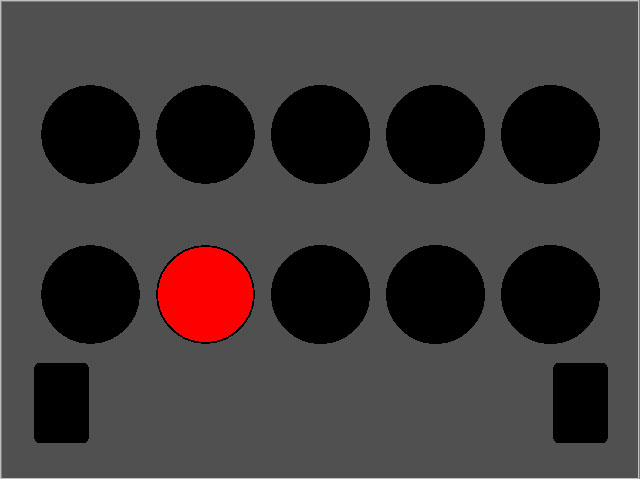
\includegraphics[width=0.7\linewidth]{images/wiener_dt}
\caption[Caption for parameters]{Wiener Determinationstest zur Überprüfung der Reaktionsfähigkeit und Belastbarkeit\footnotemark}
\label{fig:wiener_dt}
\end{figure}
\footnotetext{\label{foot:wienerdt} Schuhfried.at. (2018). SCHUHFRIED - DT. [online] Verfügbar unter: https://www.schuhfried.at/test/DT [Zugriff 28 Jan. 2018].}


\todo[inline]{Weiter Aufzählen ... }
Schwierig wird nun das Vorhaben, die genannten Tests auf dem Smartphone in App-Tests abzubilden. Diese Umsetzbarkeit wird nachfolgend im Abschnitt \ref{dataValidity} beurteilt.

Weitere Möglichkeiten der Messung bieten Wearables. Die in ihnen eingebauten Sensoren können Teile der vorher genannten Parameter direkt oder indirekt überprüfen.

\todo[inline]{Aufzählen .. }

\todo[inline]{Wichtig: Am Ende zum Ergebnis kommen, dass Zweiteilung sinnvoll ist (siehe Zwischenpräsentation)}
\todo[inline]{Hier würde sich die Tabelle der Parameter - Messung aus der Recherche gut eignen, aber aufspalten in zwei Tabellen (Smarttracking und App-Tests)!}